\documentclass[10pt]{article}
\usepackage[a4paper, margin=2cm]{geometry}
\usepackage{amsmath, amssymb}
\usepackage{lmodern}
\usepackage[T1]{fontenc}
\usepackage{enumitem}
\usepackage{graphicx}
\setlist{nosep, leftmargin=*}
\setlength{\parindent}{0pt}
\setlength{\parskip}{4pt}

\newcommand{\E}{\mathbb{E}}
\newcommand{\xo}{x^o}
\newcommand{\xm}{x^m}

\begin{document}

\begin{center}
  {\large\bfseries CFI: Alternative to PGHS}
\end{center}

\textbf{Goal:} Compute $p(y \mid \xo) = \E[\sigma(z) \mid \xo]$, $z = w^T x$, only with what the density gives tractably (for example the characteristic function $\phi_{\xm \mid \xo}$ in a PC).

\section*{PGHS problems}

Sigmoid $\to$ average of bells (Pólya-Gamma) $\to$ every bell an average of waves (Hubbard-Stratonovich):
\[
  \E[\sigma(z) \mid \xo] = \tfrac{1}{2}\, \E_{\gamma}\, \E_{u \sim \mathcal{N}(0, \gamma)} \left[ e^{\frac{1}{8\gamma}}\, e^{iu(\frac{1}{2\gamma} - w_o^T \xo)}\, \phi_{\xm \mid \xo}(-u\, w_m) \right].
\]
\begin{itemize}
  \item \textbf{Cancellation:} small $\gamma$ $\to$ huge factor $e^{1/(8\gamma)}$, fast waves, must cancel to a small value $\to$ fails numerically. Monte Carlo variant has inf. variance, quadratures only work when the scale of z is low
  \item \textbf{Depends on the scale of $z$:} it grows with the spread of $z$, i.e.\ with $\lVert w \rVert$ and the number of missing features. Works if $z$ stays small, e.g.\ with strong regularization ($C = 10^{-3}$). But we don't want to have to enforce that: it restricts the classifier.
\end{itemize}

I tried some fixes but couldn't find anything that reliably works.

\textbf{Some example attempted fixes:}
\begin{itemize}
  \item \textbf{Log space:} prevents overflow, but the problem is cancellation, not size. Large terms summing to a small value lose the result in any representation: float32 gives $10^8 + 1 - 10^8 = 0$.
  \item \textbf{No completing the square} (HS only on $e^{-\gamma z^2/2}$, this results in the moment generating function): removes $e^{1/(8\gamma)}$, but the integrand grows like $e^{z/2}$ $\to$ errors amplified for a wide $z$ (KL $\approx 10^2$ at 5000 features).
\end{itemize}

\section*{CFI: characteristic-function inversion}

Go at it from the start. What we want (the expectation of the sigmoid) and what we have (the characteristic function). Is there another way to use it for our goa l?

\begin{enumerate}[label=\textbf{\arabic*.}, ref=\arabic*, itemsep=6pt]

\item \label{step:cf-z} \textbf{CF of $z$:} $\phi_z(s) = \E[e^{isz} \mid \xo]$. $z$ is only random through the missing features; with $z = w_o^T \xo + w_m^T \xm$ the observed part is a constant and factors out:
\begin{align*}
  \phi_z(s) = \E[e^{isz} \mid \xo] &= \E[e^{is(w_o^T \xo + w_m^T \xm)} \mid \xo] \\
  &= e^{is\, w_o^T \xo}\, \E[e^{i (s w_m)^T \xm} \mid \xo] \\
  &= e^{is\, w_o^T \xo}\, \phi_{\xm \mid \xo}(s\, w_m).
\end{align*}

\item \label{step:cf-sigmoid} \textbf{CF of the sigmoid:} $\sigma$ is the CDF of the logistic distribution, $\sigma(t) = P(L \leq t)$. So the LR predicts $1$ when $z$ exceeds a random threshold $L$, and with $z$ random too, the expected prediction is a probability ($L$ independent of $x$, continuous):
\begin{align*}
  \E[\sigma(z) \mid \xo] &= \E[P(L \leq z \mid z) \mid \xo] \\
  &= P(L \leq z \mid \xo).
\end{align*}
The CF of the logistic distribution is known in closed form, real and even:
\[
  \phi_L(s) = \frac{\pi s}{\sinh(\pi s)}.
\]

\item \label{step:cf-difference} \textbf{CF of $z - L$:} Gil-Pelaez (step~\ref{step:gil-pelaez}) gives probabilities of the form $P(Y > 0)$ from the CF of $Y$. So we write $P(L \leq z \mid \xo) = P(z - L > 0 \mid \xo)$, i.e.\ $Y = z - L$. Now we need its CF. We know the CF of $z$ (step~\ref{step:cf-z}) and of $L$ (step~\ref{step:cf-sigmoid}), and because $z$ and $L$ are independent, the CF of $z - L$ can be built from these two:
\begin{align*}
  \phi_{z-L}(s) = \E[e^{is(z - L)} \mid \xo] &= \E[e^{isz}\, e^{-isL} \mid \xo] \\
  &= \E[e^{isz} \mid \xo]\, \E[e^{-isL}] \\
  &= \phi_z(s)\, \phi_L(-s) \\
  &= \phi_z(s)\, \frac{\pi s}{\sinh(\pi s)}.
\end{align*}

\item \label{step:gil-pelaez} \textbf{Gil-Pelaez inversion:} a formula that gives the probability that a variable $Y$ is positive from its CF alone:
\[
  P(Y > 0) = \frac{1}{2} + \frac{1}{\pi} \int_0^\infty \frac{\mathrm{Im}\, \phi_Y(s)}{s} \, \mathrm{d}s.
\]
We set $Y = z - L$ and insert its CF from step~\ref{step:cf-difference}. The factor $\frac{\pi s}{\sinh(\pi s)}$ is real, so it can be moved out of $\mathrm{Im}$, and then its $s$ cancels with the $\frac{1}{s}$ and its $\pi$ with the $\frac{1}{\pi}$:
\begin{align*}
  \E[\sigma(z) \mid \xo] = P(z - L > 0 \mid \xo) &= \frac{1}{2} + \frac{1}{\pi} \int_0^\infty \frac{1}{s}\, \mathrm{Im} \left[ \phi_z(s)\, \frac{\pi s}{\sinh(\pi s)} \right] \mathrm{d}s \\
  &= \frac{1}{2} + \frac{1}{\pi} \int_0^\infty \frac{1}{s}\, \frac{\pi s}{\sinh(\pi s)}\, \mathrm{Im}\, \phi_z(s) \, \mathrm{d}s \\
  &= \frac{1}{2} + \int_0^\infty \frac{\mathrm{Im}\, \phi_z(s)}{\sinh(\pi s)} \, \mathrm{d}s.
\end{align*}

\end{enumerate}

$P(z - L > 0 \mid \xo)$ is the probability that the label is $1$, so exactly what we want.

\textbf{Intuition:} the sigmoid is a weighted sum of sine waves ($\frac{1}{\sinh(\pi s)}$). The expectation replaces each wave by its expectation $\mathrm{Im}\, \phi_z(s)$, which the PC gives.

\textbf{Properties:}
\begin{itemize}
  \item exact up to the trapezoid rule, one-dimensional;
  \item only the characteristic function and the mean and variance of $z$;
  \item no sign flip, no special quadrature, no amplification ($|\phi_z| \leq 1$);
  \item independent of the scale of $z$, so no regularization needed;
  \item deterministic and differentiable in $w$ and the density $\to$ joint training on incomplete data (PCLR).
\end{itemize}

\clearpage
\textbf{Results:}

Only 40 frequencies (evaluations of the CF) for the first plot. Against 1000 samples for the conditional sampling. KL against ground truth (closed form for GMM). The last figure is an older one where PGHS (called PCPG) and the CFI (called Gil-Paleaz) were compared directly.
\begin{center}
  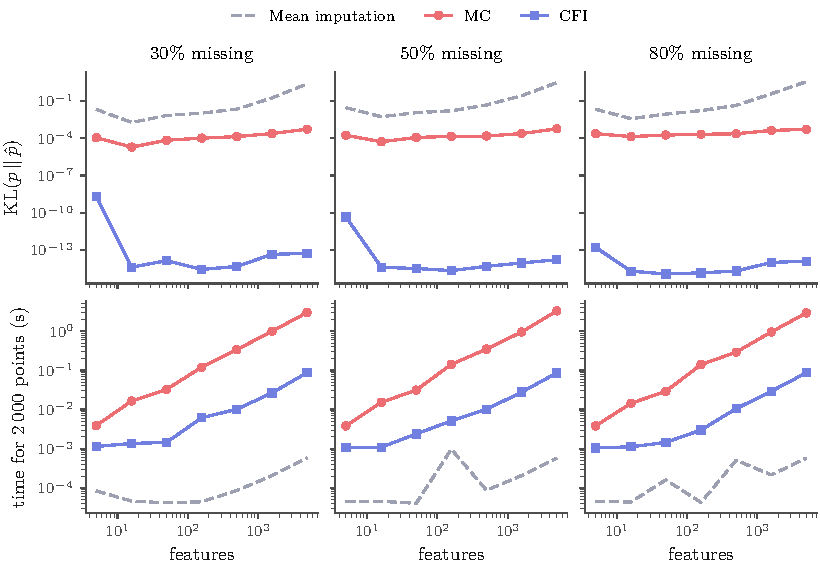
\includegraphics[width=0.85\textwidth]{../thesis/figures/estimate/gmm/comparison_0.5_1000_40.pdf}

  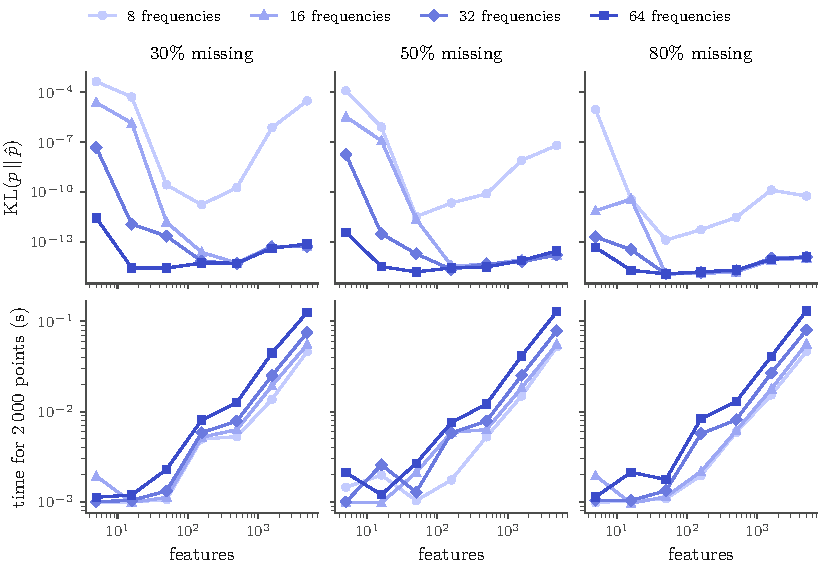
\includegraphics[width=0.85\textwidth]{../thesis/figures/estimate/gmm/cfi_frequencies_0.5_1000_40.pdf}

  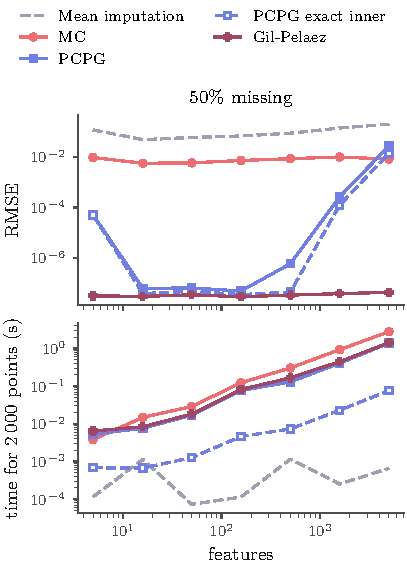
\includegraphics[width=0.85\textwidth]{../code/figures/estimate/gmm/old/estimate_pghs_gp.pdf}
\end{center}

\end{document}
